
\subsection{Desired properties of a chemistry benchmark} \label{sec:desired-properties}

\begin{itemize}
    \item \emph{End-to-end automation}. For model development, the evaluations must be run many times (e.g., on regular intervals of a training run).
    Approaches that rely on humans scoring the answers of a system\autocite{Schulze_Balhorn_2024, ai4science2023impact, castro2023large} can thus not be used.
    \item \emph{Careful validation by experts}. Manual curation is needed to minimize the number of incorrect or unanswerable questions.\autocite{northcutt2021pervasive}
    This is motivated by the observation that many widely used benchmarks are plagued by noisiness.\autocite{Frye_2023, Awg}
    \item \emph{Usable with models that support special treatment of molecules}. Some models, such as Galactica\autocite{taylor2022galactica}, use special tokenization or encoding procedures for molecules or equations.
    The benchmark system must encode the semantic meaning of various parts of the question or answer to support this.
    \item \emph{Usable with black box systems}. Many relevant systems do not provide access to model weights or raw logits.
    This might be the case because the systems are proprietary or because they involve not only \glspl{llm} but also external tools such as search \glspl{api} or code executors.\autocite{schick2024toolformer, karpas2022mrkl, yao2022react}
    Thus, a benchmark should not assume access to the raw model outputs but be able to operate on text completions.
    \item \emph{Probing capabilities beyond answering of \glspl{mcq}}. In real-world chemistry, as well as higher-level university education, multiple-choice questions are seldom utilized.
    Yet, most benchmarking frameworks focus on the \gls{mcq} setting because of the ease of evaluation. Realistic evaluations must measure capabilities beyond answering \gls{mcq}.
    \item \emph{Cover a diverse set of topics}. Chemistry, as the \enquote{central science}, bridges multiple disciplines.\autocite{Aspuru_Guzik_2018} To even just approximate \enquote{chemistry capabilities} the topics covered by a chemistry benchmark must be very diverse.
    \item \emph{Cover diverse skills}. To holistically judge performance it is important to cover questions relying on reasoning, calculation, knowledge, and intuition.
    \item \emph{Cover a range of difficulty levels}. To allow for a continuous measure of improvement for a range of different (evolving) systems, a benchmark should cover a wide range of difficulty levels.
    \item \emph{Impossible to completely solve with current models}. A benchmark should contain questions that are impossible to solve with current models. If current models can solve all questions, the benchmark provides no useful signal.
\end{itemize}

\subsection{Related work}
Existing benchmarks such as those from \textcite{guo2023large}, \textcite{sun2023scieval}, \textcite{Schulze_Balhorn_2024}, \textcite{Cai_2024} fail to comply with most of the requirements stipulated above.
While these benchmarks could provide valuable insights in the short term, they cannot follow the rapid additions to the \gls{llm} space.
\chembench aims to correct this through a set of developments: compatibility with BigBench, end-to-end automation, a particular focus on chemical safety, employment of diverse prompting strategies, and specialized notation for molecules and mathematical symbols.
Moreover, our robust framework, including the platform \url{chembench.org}, will engage the community in open-source contributions.

\clearpage
\subsection{Benchmark corpus}
To ensure maximal interoperability with existing benchmarks or tools, we curated the data in an extended form of the widely used BigBench format.\autocite{srivastava2022beyond}
This also implies that future baselines can be built on top of our infrastructure if saved in the same format.

\subsubsection{Curation workflow}
Questions were added via pull requests to the \chembench repository on GitHub.
This allowed for a manual review of each question by expert reviewers (with backgrounds in chemistry, materials science, chemical engineering, and physics).
The reviews were conducted directly on the GitHub platform, where our entire curation history is also publicly available.

The general guidelines followed by the reviewer are the following:

\begin{itemize}
    \item \textbf{Originality:} Questions should not be readily findable online or in other easily accessible sources (example \url{https://github.com/lamalab-org/chem-bench/pull/392#discussion_r1694299474})
    \item \textbf{Ambiguity:} Questions with unclear wording or multiple interpretations (example \url{https://github.com/lamalab-org/chem-bench/pull/420#discussion_r1698147159} )
    \item \textbf{Factual or heuristic Errors: }Questions containing factual inaccuracies or misconceptions are not included (example \url{https://github.com/lamalab-org/chem-bench/pull/389#discussion_r1686187301})
    \item \textbf{Clarity and Difficulty: } They should pose a challenge and encourage exploration within the chemical domain (example \url{https://github.com/lamalab-org/chem-bench/pull/391#discussion_r1679276714})
    \item \textbf{Out of Scope:} Questions outside the realm of chemistry are rejected.
    \item \textbf{Contribution to Dataset Diversity: }Questions should cover a wide range of chemical concepts and sub-disciplines. They should add value by expanding the breadth of the dataset. That is, questions already multiple (>10) times in the corpus in a similar form are rejected.
\end{itemize}

Reviewers also solved the questions to verify the answers. They also performed web searches to ensure questions were not easily found online. The reviewers often guided the revision process to ensure the question aligned with the guidelines. Questions that don't meet the criteria are either rejected or suggested for revision and most often, they are modified to a new question. Reviewers also provide feedback on the skill and difficulty annotations.

In addition to the manual review, we also performed automated checks to ensure the quality of the questions. The schemas, Latex templating, and other formatting aspects are checked automatically using GitHub Actions.

While adding questions from existing benchmarks might seem to be another good source of semi-automatically generated data, we prioritized the diversity of the data and avoided data contamination while addressing the guidelines above and in \Cref{sec:desired-properties}.
However, even though we decided not to include questions from other previously published chemistry-focused benchmarks into the \chembench corpus, the framework is flexible enough to be readily extended with questions from other benchmarks.

\subsubsection{Composition}

\Cref{fig:cb_humanset} shows the distribution of topics and required skills in the human subset of the \chembench corpus.

\begin{figure}
    \centering
    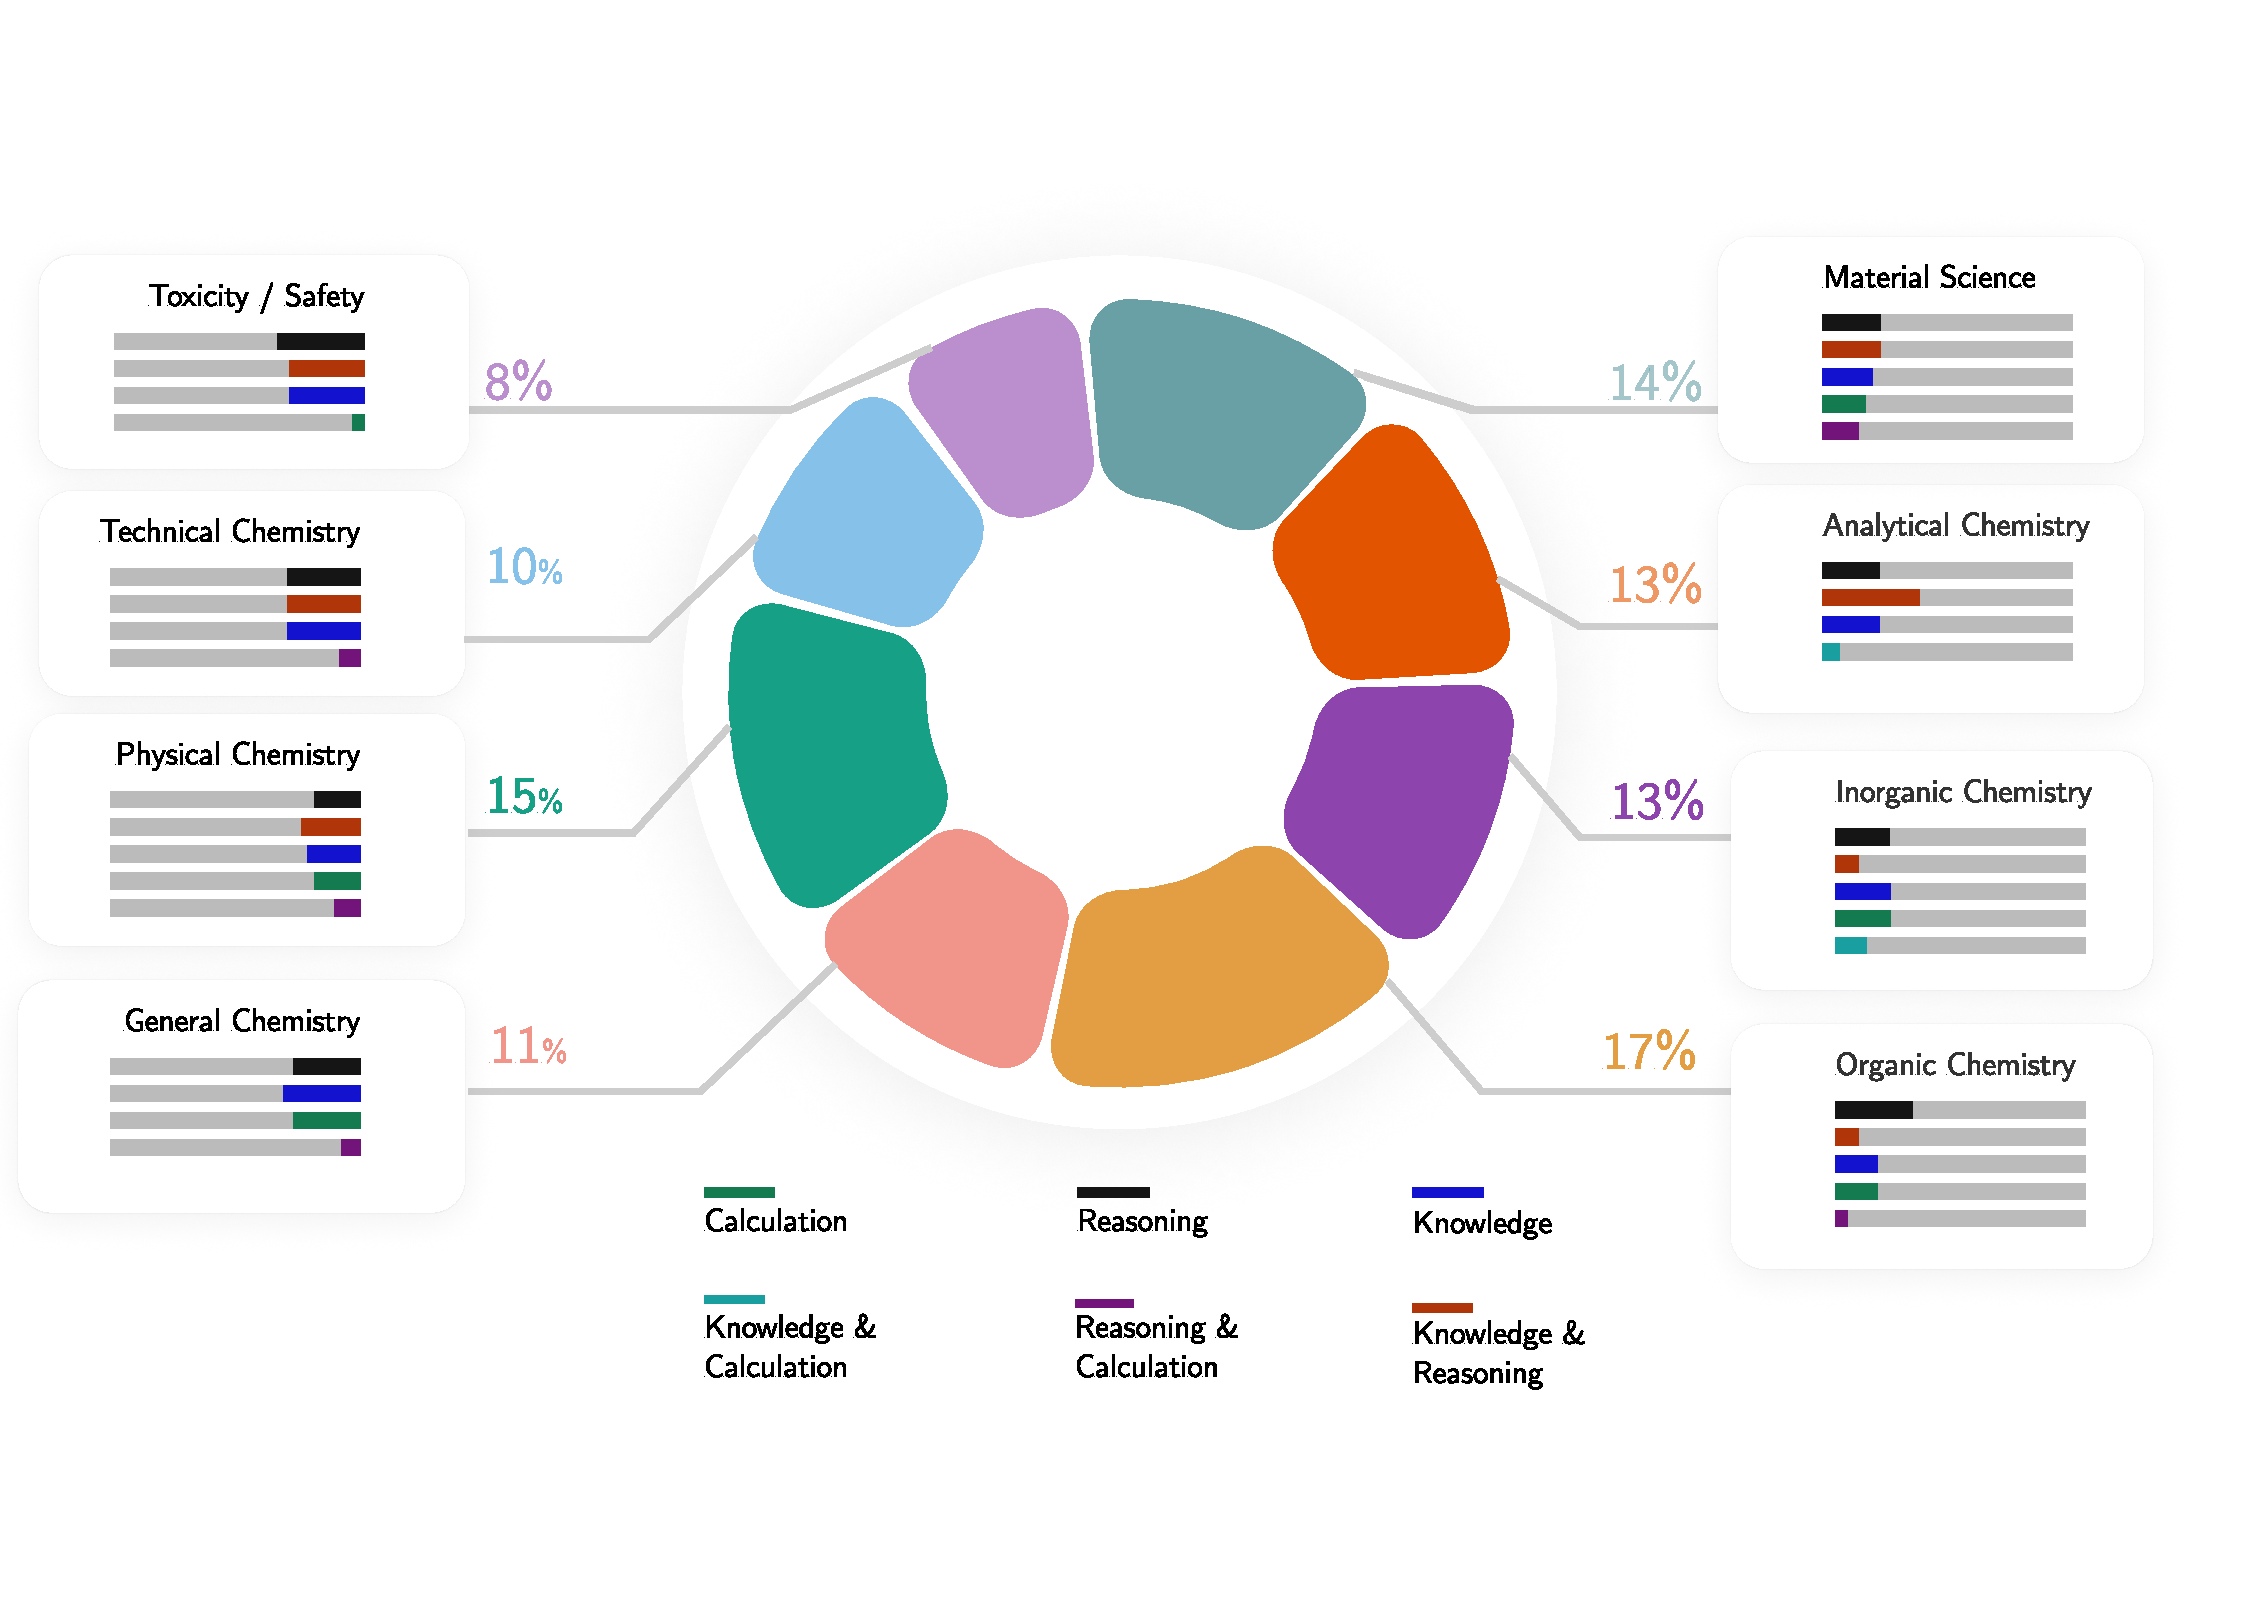
\includegraphics[width=\textwidth]{figures/CB_HUMANSET_FIG_V1.pdf}
    \caption{\textbf{Composition of the human subset.} The circular plot shows the distribution of topics and required skills in the human subset of the \chembench corpus. The human subset is a representative subset of the full corpus, with a balanced distribution of topics and skills.}
    \label{fig:cb_humanset}
\end{figure}

The corpus of the questions in \chembench, as shown in \Cref{tab:chembench_corpus_topic}, can be divided according to which chemical topic they belong to.

\begin{table}
    \centering
    \small
    \caption{\textbf{Examples for each of the topics considered in the evaluation of the \chembench corpus.} The table shows the percentage of questions in the corpus that belong to each topic, as well as example questions.} \\
    \label{tab:chembench_corpus_topic}
    {\fontsize{8}{9}\selectfont
        \begin{tabularx}{\textwidth}{X}
            \toprule
            \multicolumn{1}{c}{\textbf{Analytical Chemistry} 166 Questions (5.8\%)} \\
            \midrule
            Which of the following analytical methods is most appropriate for performing a survey analysis of a solid sample containing various metals? \\
            A. X-ray fluorescence analysis \\
            B. Differential pulse polarography \\
            C. Flame-atomic absorption spectroscopy \\
            D. Gas chromatography with flame ionization detector \\
            E. Hydride generation atomic absorption spectroscopy \\
            \midrule
            \multicolumn{1}{c}{\textbf{Chemical Preference} 1001 Questions (35\%)} \\
            \midrule
            Imagine an early virtual screening campaign setting (accounting for simple aspects such as oral availability and small molecular profile, but no other modalities such as covalency or bifunctionality). Which of the following two candidates would you prefer for further development? \\
            [START\_SMILES]N\#Cc1ccc(OCCCN2CC3CN\-(CCNS(=O)(=O)c4ccc(F)cc4)CC(C2)O3)cc1\-[END\-\_SMILES] \\
            [START\_SMILES]O=C1CC(c2ccc(CC(NS(=O)\-(=O)\-c3cc(Cl)cc(Cl)c3)c3nc4ccccc4[nH]3)cc2)S\-(=O)\-(=O)N1[END\_SMILES] \\
            \midrule
            \multicolumn{1}{c}{\textbf{General Chemistry} 152 Questions (5.3\%)} \\
            \midrule
            Which of the following salts is an acidic salt? \\
            A. \ce{NH4Cl} \\
            B. \ce{Na2CO3} \\
            C. \ce{NaH2PO4} \\
            D. \ce{Zn(OH)Cl} \\
            \midrule
            \multicolumn{1}{c}{\textbf{Inorganic Chemistry} 94 Questions (3.3\%)} \\
            \midrule
            What is the oxidation number of the metal in the compound \ce{[ZrF7]^{3-}}\\
            \midrule
            \multicolumn{1}{c}{\textbf{Materials Science} 89 Questions (3.1\%)} \\
            \midrule
            For NMR analysis, you need to digest the MOF in a strong acid to remove the linker and leave the metal clusters intact. Why would one choose \ce{HF} over \ce{HCl} for this purpose? \\
            A. \ce{F-} forms a stable bonds to the metal ions \\
            B. \ce{HF} has a better water solubility than \ce{HCl} \\
            C. \ce{HF} has a higher boiling point than \ce{HCl} \\
            D. \ce{HF} is a weaker acid than \ce{HCl} \\
            \midrule
            \multicolumn{1}{c}{\textbf{Organic Chemistry} 441 Questions (15.5\%)} \\
            \midrule
            What is the reaction mechanism that describes the following reaction (represented using reaction SMILES) [START\_RXNSMILES]CCCl.CO[Na]>>[Na]Cl.CCOC\-[END\_RXNSMILES]? \\
            A. $E_1$ \\
            B. $E_{cb}$ \\
            C. $S_N1$ \\
            D. $S_N2$ \\
            \midrule
            \multicolumn{1}{c}{\textbf{Physical Chemistry} 179 Questions (6.3\%)} \\
            \midrule
            The Born-Oppenheimer (BO) approximation is widely used in computational chemistry, but its accuracy can vary depending on the system. Among the following options, for which system is the Born-Oppenheimer approximation likely to be least applicable? \\
            A. \ce{C60} \\
            B. \ce{CH4} \\
            C. \ce{Fe(CO)5} \\
            D. \ce{H2+} \\
            E. \ce{NaCl} \\
            \midrule
            \multicolumn{1}{c}{\textbf{Technical Chemistry} 42 Questions (1.5\%)} \\
            \midrule
            Which of the following statements is true about the different types of ideal reactors? \\
            A. In a batch reactor, the composition is uniformly mixed and remains the same throughout the reactor and at the exit \\
            B. In a batch reactor, the fluid passes through the reactor with no mixing of earlier and later entering fluid \\
            C. In a mixed flow reactor, the composition changes with time but is uniform everywhere within the reactor \\
            D. In a plug flow reactor, the fluid moves in single flow through the reactor with no mixing and no overtaking \\
            \midrule
            \multicolumn{1}{c}{\textbf{Toxicity/Safety} 690 Questions (24.2\%)} \\
            \midrule
            Pindolol and propranolol are (relatively nonselective) antagonists at $\beta_1$- and $\beta_2$-adrenoceptors. However, pindolol is a partial agonist, whereas propranolol is a pure antagonist. What follows from this? \\
            A. Pindolol has a greater therapeutic range than propranolol \\
            B. Pindolol has a longer half-life than propranolol \\
            C. Pindolol has intrinsic activity \\
            D. Pindolol is more lipophilic than propranolol \\
            E. Pindolol is more potent than propranolol \\
            \bottomrule
        \end{tabularx}
    }
\end{table}

\normalsize


In addition, as shown in \Cref{tab:cb_skillset} the \chembench corpus can be divided considering the different skills needed to solve the questions. The plot shows a balanced distribution of the required skills in the \chembench corpus. \Cref{tab:cb_skillset} shows an example question for each skill category.

\begin{figure}
    \centering
    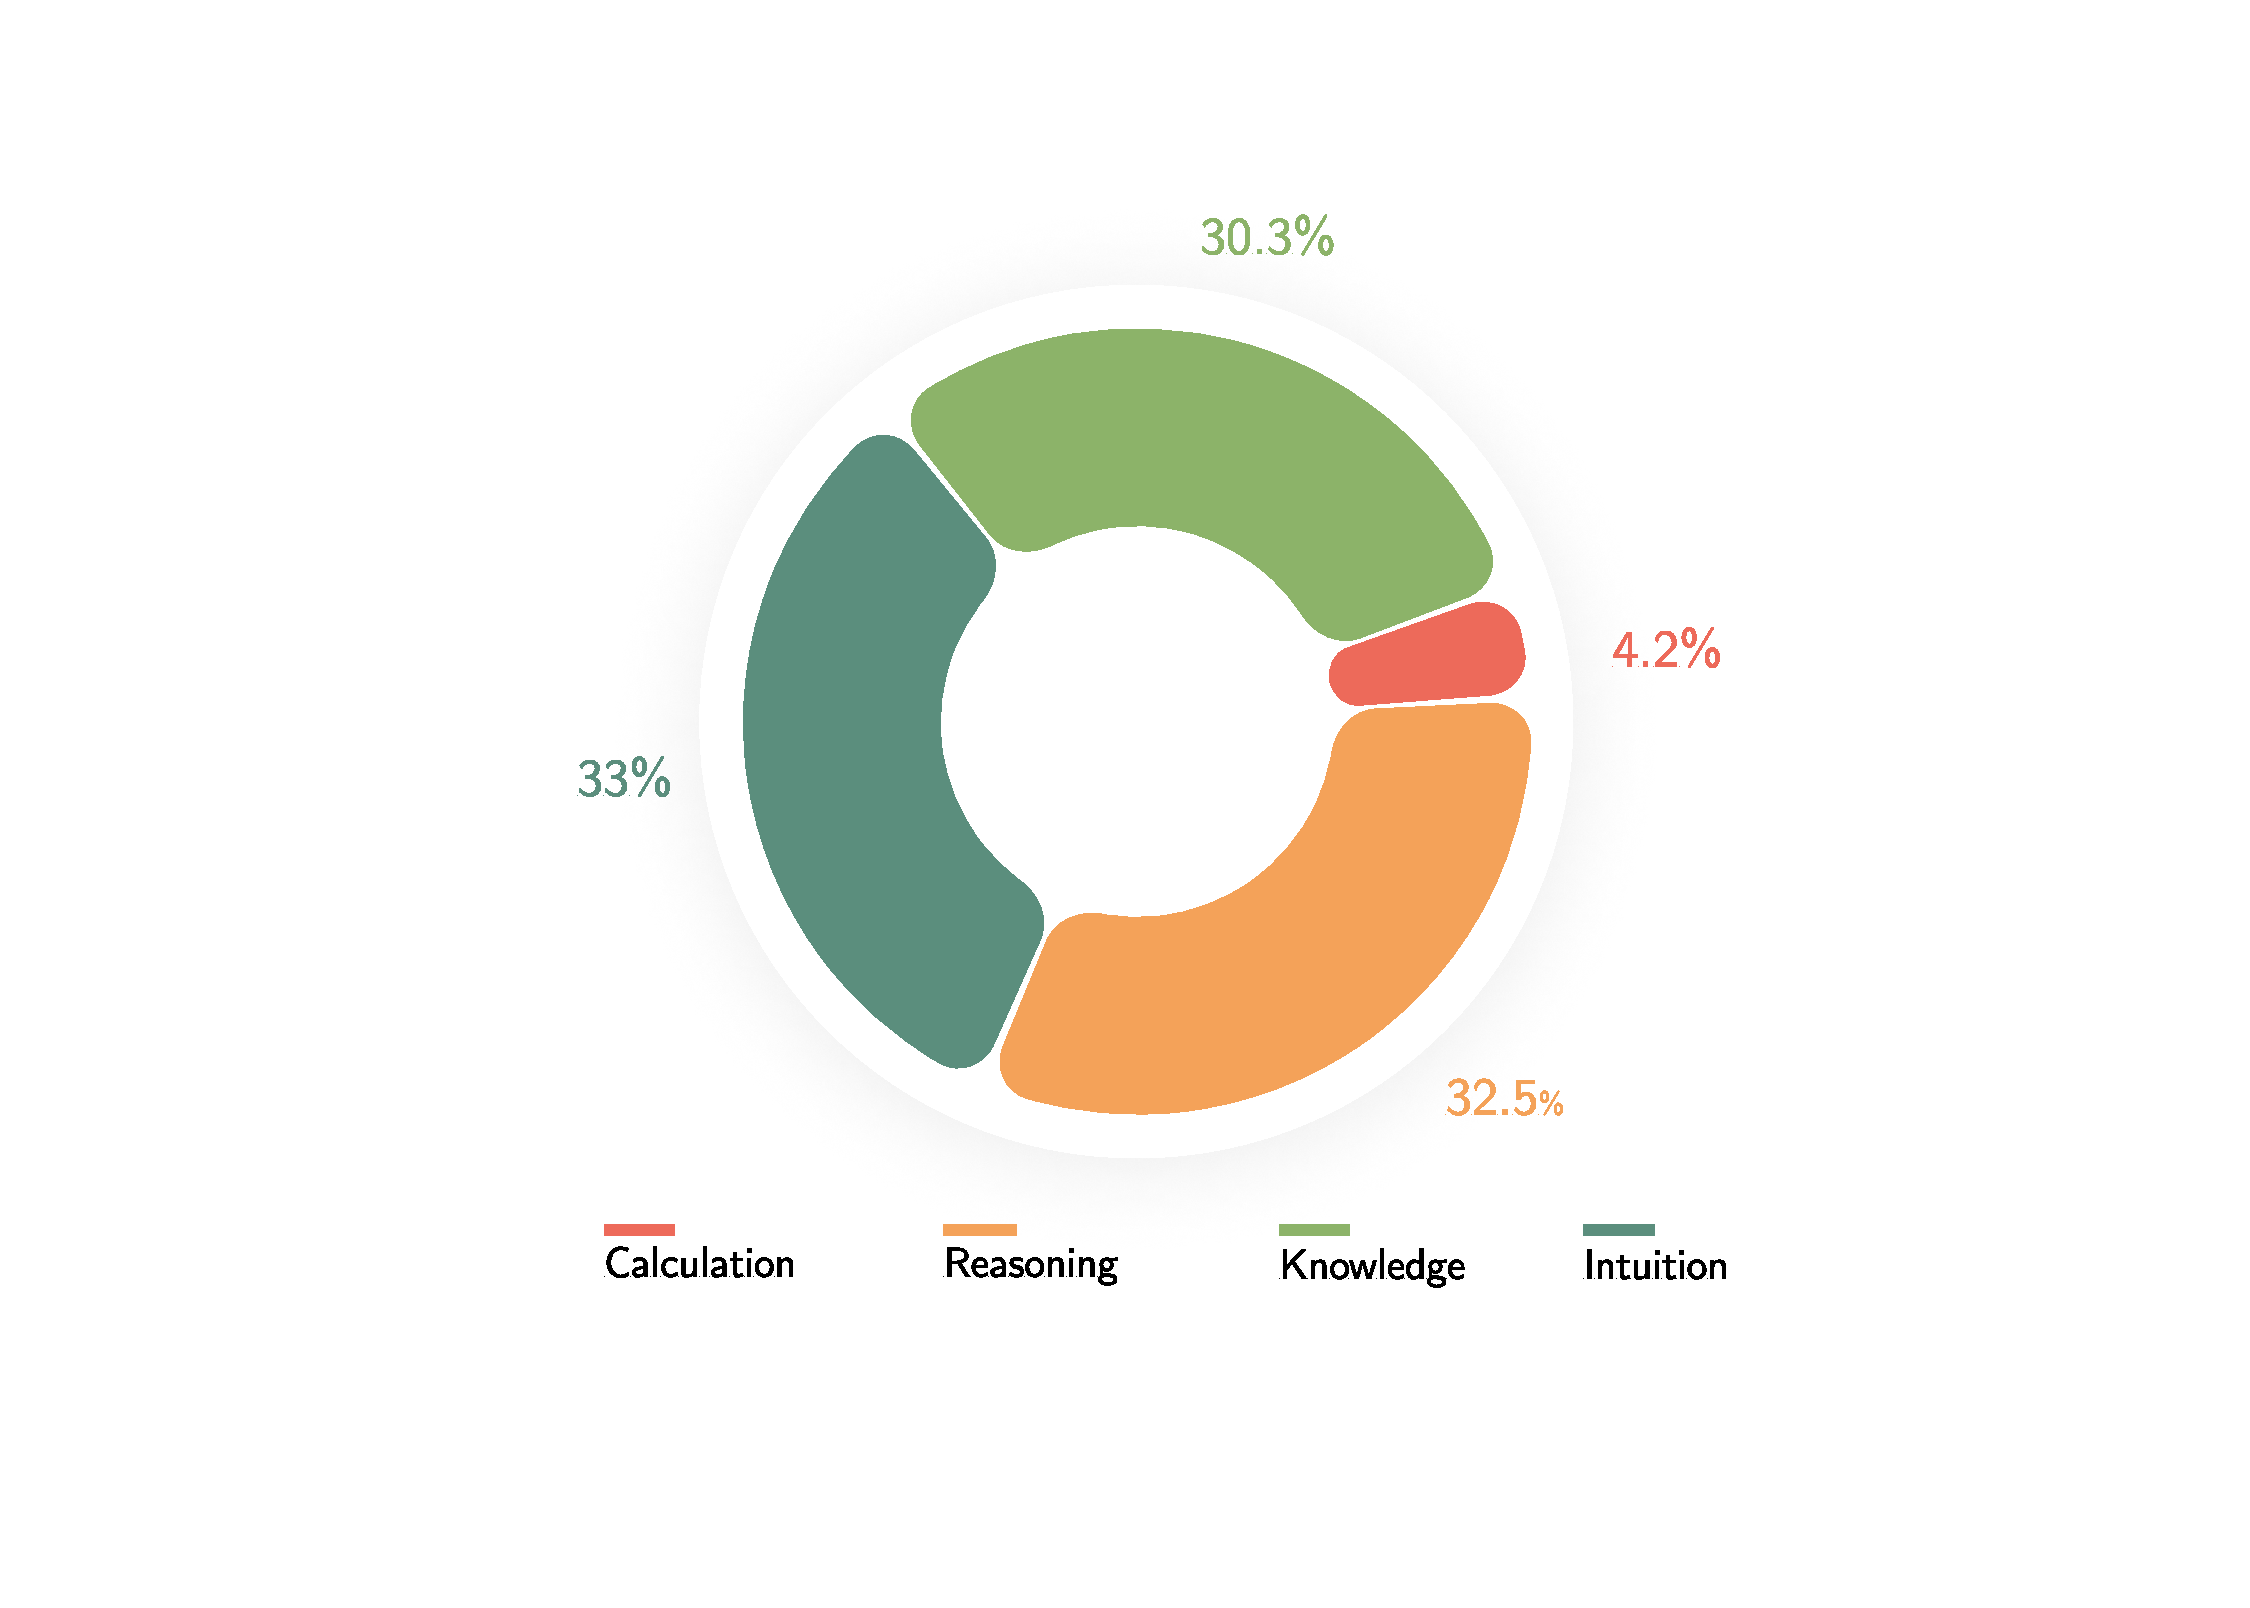
\includegraphics[width=\textwidth]{figures/CB_SKILL_FIG_V1.pdf}
    \caption{\textbf{Composition of the required skills considered in the \chembench corpus.} The circular plot shows the distribution of required skills in the \chembench corpus.}
    \label{fig:cb_skillset}
\end{figure}


\begin{table}
    \centering
    \small
    \caption{\textbf{Examples for each of the required skills considered in the \chembench corpus.} The table shows the number of questions for each skill and an example question. Note that the total count in this table is bigger than the \chembench corpus. This is because the same question can be annotated with two different \enquote{requires} skills, i.e. Reasoning and Calculation.} \\
    \label{tab:chembench_corpus_cognitive}
    {\fontsize{8}{9}\selectfont
        \begin{tabularx}{\textwidth}{X}
            \toprule
            \multicolumn{1}{c}{\textbf{Knowledge} 919 Questions} \\
            \midrule
            Which of the following salts is an acidic salt? \\
            A. \ce{NH4Cl} \\
            B. \ce{Na2CO3} \\
            C. \ce{NaH2PO4} \\
            D. \ce{Zn(OH)Cl} \\
            \midrule
            \multicolumn{1}{c}{\textbf{Reasoning} 987 Questions} \\
            \midrule
            How can the optical impact of quantum confinement on the electronic structure of a quantum dot be observed experimentally? \\
            A. By atomic force microscopy \\
            B. By transform infrared spectroscopy \\
            C. By measuring a photoluminescence spectrum \\
            D. By absorption spectroscopy \\
            \midrule
            \multicolumn{1}{c}{\textbf{Intuition} 1001 Questions} \\
            \midrule
            Imagine an early virtual screening campaign setting (accounting for simple aspects such as oral availability and small molecular profile, but no other modalities such as covalency or bifunctionality). Which of the following two candidates would you prefer for further development? \\
            A. [START\_SMILES]CC1(C)Oc2ccc([N+](=O)[O-])cc2[C@@H](N2CCOCC2)[C\@\@H]1O[END\_SMILES] \\
            B. [START\_SMILES]Cc1ccccc1N=C(S)N1CCC(NC\-(=O)c2ccco2)CC1[END\_SMILES] \\
            \midrule
            \multicolumn{1}{c}{\textbf{Calculation} 128 Questions} \\
            \midrule
            Given that the average molar mass of the polymer chains in this sample of poly(lactic acid) (PLA) is \SI{595}{g mol^{-1}} using end-group analysis, where \SI{0.1619}{g} of PLA was dissolved in \SI{25}{cm^3} of benzyl alcohol and titrated with \SI{0.0400}{mol dm^{-3}} \ce{KOH} solution. The volume of \ce{KOH} solution required to reach the endpoint was \SI{6.81}{cm^3}. What is the average number of monomer units in each polymer chain of this sample? \\
            \bottomrule
        \end{tabularx}
    }
\end{table}

\normalsize

In analyzing the performance of state-of-the-art models on the ChemBench corpus, we identified several chemical topics where the models consistently struggled to provide correct answers. The following table \cref{tab:chembench_corpus_models_failed_topic} presents examples of challenging questions across different chemical domains, highlighting specific areas where current models need improvement

\begin{table}
    \centering
    \small
    \caption{\textbf{Examples of topics evaluated in the \chembench corpus that the state-of-the-art model failed to answer correctly.} The table displays the percentage of questions in the corpus for each topic, along with example questions and the percentage of questions that were not answered correctly by the models.} \\
    \label{tab:chembench_corpus_models_failed_topic}
    {\fontsize{8}{9}\selectfont
        \begin{tabularx}{\textwidth}{X}
            \toprule
            \multicolumn{1}{c}{\textbf{Analytical Questions} 166 Questions (5.8\%) (26.5\%)} \\
            \midrule
            Which of the following methods can be used to support the structure elucidation of planar molecules by examining the topography of individual molecules? \\
            A. DESI-mass spectrometry \\
            B. XPS \\
            C. atomic force microscopy \\
            D. scanning tunneling microscopy \\
            E. secondary ion mass spectrometry \\
            \midrule
            \multicolumn{1}{c}{\textbf{Chemical Preference} 1001 Questions (35\%) (8.5\%)} \\
            \midrule
            Imagine an early virtual screening campaign setting (accounting for simple aspects such as oral availability and small molecular profile, but no other modalities such as covalency or bifunctionality). Which of the following two candidates would you prefer for further development? \\
            [START\_SMILES]N\#Cc1ccc(OCCCN2CC3CN\-(CCNS(=O)(=O)c4ccc(F)cc4)CC(C2)O3)cc1\-[END\-\_SMILES] \\
            [START\_SMILES]O=C1CC(c2ccc(CC(NS(=O)\-(=O)\-c3cc(Cl)cc(Cl)c3)c3nc4ccccc4[nH]3)cc2)S\-(=O)\-(=O)N1[END\_SMILES] \\
            \midrule
            \multicolumn{1}{c}{\textbf{General Chemistry} 152 Questions (5.3\%) (3.2\%)} \\
            \midrule
            Why \ce{SCl6} does not exist if other similar molecules such as \ce{SF6} exist? \\
            A. \ce{SCl6} does not exist because of steric effects \\
            B. \ce{SCl6} does not exist because of the high electronegativity of chlorine \\
            C. \ce{SCl6} does not exist because of the high ionization potential of the chlorine \\
            D. \ce{SF6} exist because of the high electronegativity of fluorine \\
            \midrule
            \multicolumn{1}{c}{\textbf{Inorganic Chemistry} 94 Questions (3.3\%) (4.2\%)} \\
            \midrule
            What is the spin-only magnetic moment (in units of Bohr-magnetons) for the low-spin case of the metal complex \ce{RhCl(CO)(PPh3)2}?\\
            \midrule
            \multicolumn{1}{c}{\textbf{Materials Science} 89 Questions (3.1\%) (0.9\%)} \\
            \midrule
            What are the conditions for the observation of effects of quantum confinement in quantum dots? \\
            A. All dimension of the material must be smaller than exciton Bohr radius \\
            B. One dimension of the quantum dot must be smaller than exciton Bohr radius \\
            C. The movement od charge carriers is limited in all spatial dimensions \\
            \midrule
            \multicolumn{1}{c}{\textbf{Organic Chemistry} 441 Questions (15.5\%) (0.5\%)} \\
            \midrule
            What makes acrylates more reactive than typical hydrocarbons? \\
            A. The carbonyl group \\
            B. The double bond \\
            C. The hydroxyl group \\
            D. The vinyl group \\
            \midrule
            \multicolumn{1}{c}{\textbf{Physical Chemistry} 179 Questions (6.3\%) (13.4\%)} \\
            \midrule
            Why are polar molecules more soluble in water than non-polar molecules? \\
            A. Non-polar molecules should break hydrogen bonds in water to dissolve \\
            B. The entropy of the system increases when non-polar molecules dissolve in water \\
            C. Water has a dipole and can easier isolate polar molecules from each other \\
            D. Water makes stable dipole-dipole interactions with polar molecules \\
            \midrule
            \multicolumn{1}{c}{\textbf{Technical Chemistry} 42 Questions (1.5\%) (4.7\%)} \\
            \midrule
            Which of the following statements is/are true about granulation shaping of solid catalysts? \\
            A. Broader product diameter distribution than pellets or extrudates \\
            B. Facilitates reactor upscaling \\
            C. It is also called snow-ball \\
            D. Not suitable to prepare egg-shell catalysts \\
            \midrule
            \multicolumn{1}{c}{\textbf{Toxicity/Safety} 690 Questions (24.2\%) (40.4\%)} \\
            \midrule
            What determines the flammability of polyols? \\
            A. Their chemical structure \\
            B. Their low volatility \\
            C. Their odor threshold \\
            D. Their reaction with acids \\
            \bottomrule
        \end{tabularx}
    }
\end{table}

\normalsize

To better understand the cognitive demands of chemical assessment, we categorized the questions in the ChemBench corpus according to the primary skills required to solve them. The table \Cref{tab:chembench_corpus_models_failed_cognitive} below shows representative examples of questions that state-of-the-art models failed to answer correctly across different cognitive skill categories, including knowledge, reasoning and intuition.
\begin{table}
    \centering
    \small
    \caption{\textbf{Examples of required skills evaluated in the \chembench corpus that the state-of-the-art model failed to answer correctly} The table displays the number of questions for each skill, along with an example question that the model failed to answer.} \\
    \label{tab:chembench_corpus_models_failed_cognitive}
    {\fontsize{8}{9}\selectfont
        \begin{tabularx}{\textwidth}{X}
            \toprule
            \multicolumn{1}{c}{\textbf{Knowledge} 919 Questions} \\
            \midrule
            Which of the following are true for phosphoric acid? \\
            A. Is a weak acid, so it is not toxic \\
            B. Should never be tasted \\
            C. Though a component of soft drinks, reacts vigorously with water when in concentrated form \\
            \midrule
            \multicolumn{1}{c}{\textbf{Reasoning} 987 Questions} \\
            \midrule
            Which of the following elements has the largest atomic radius? \\
            A. \ce{Fr} \\
            B. \ce{He} \\
            C. \ce{Li} \\
            D. \ce{Rb} \\
            \midrule
            \multicolumn{1}{c}{\textbf{Intuition} 1001 Questions} \\
            \midrule
            Imagine an early virtual screening campaign setting (accounting for simple aspects such as oral availability and small molecular profile, but no other modalities such as covalency or bifunctionality). Which of the following two candidates would you prefer for further development? \\
            A. [START_SMILES]CCc1c(CCOC)nn(-c2ccccc2)c1-c1ccccc1[END_SMILES] \\
            B. [START_SMILES]Cc1cc(/C=C2\\C(=N)N3N=C(S(C)(=O)=O)SC3=NC2=O)c(C)n1Cc1ccccc1[END_SMILES] \\
            \midrule
            \multicolumn{1}{c}{\textbf{Calculation} 128 Questions} \\
            \midrule
            The cell potential for the overall cell reaction during electrolysis of water, \ce{2H2O(l) -> 2H2(g) + O2(g)} is \SI{-1.23 V}. What is the standard electrode potential for the half reaction, \ce{2H2O(l) -> O2(g) + 4H+(aq) + 4e-} in V? \\
            \bottomrule
        \end{tabularx}
    }
\end{table}

\normalsize




\clearpage
\subsection{Model performance} \label{sec:model_performance_app}
We also evaluated the model performance on the entire \chembench corpus.
\Cref{fig:barplot_all_correct_all_questions} shows the fraction of questions that were answered correctly by the models.

\begin{figure}[htb]
    \centering
    \includegraphics{figures/overall_performance.pdf}
    \caption{\textbf{Overall performance of the models on the \chembench corpus.} The bar plot shows the fraction of questions that were answered correctly by the models. Scores computed on the entire \chembench corpus.}
    \label{fig:barplot_all_correct_all_questions}
    \script{plot_overview_performance_plot.py}
\end{figure}

\Cref{fig:all_questions_models_completely_correct_radar_overall} shows the performance of the models on the different topics of the \chembench corpus.
The general pattern of performance varies significantly between the different topics and is also observed when the models are evaluated on the entire corpus.
However, since some subjects are composed of questions from different sources, the ranking of the models is, in some instances, different from the one on \chembenchmini.

\begin{table}
    \caption{\textbf{Performance of the models on the \chembench corpus.} The table shows the fraction of questions answered correctly by the models for different skills and difficulty levels. Models with \enquote{T-one} in the name were run for a temperature of 1, which allows us to study the temperature effect in the benchmark. Systems with \enquote{ReAct} in the name are tool augmented, i.e., they can call external tools such as web search or a calculator to answer the questions better. However, we limit those systems to ten calls to the \gls{llm}. This constraint often led the systems to not find the correct answer within the specified number of calls. In this case, we consider the answer as incorrect (see \Cref{sec:react-environment}).}
    \resizebox{\textwidth}{!}{
    \variable{output/performance_table.tex}
    }
    \label{tab:performance_table}
\end{table}

\begin{table}
    \caption{\textbf{Performance of the models on \chembenchmini.} The table shows the fraction of questions answered correctly by the models for different skills and difficulty levels.}
    \resizebox{\textwidth}{!}{
    \variable{output/performance_table_human_subset.tex}
    }
    \label{tab:performance_table_human_subset}
\end{table}

\begin{figure}[htb]
    \centering
    \includegraphics[width=\textwidth]{figures/all_questions_models_completely_correct_radar_overall.pdf}
    \caption{\textbf{Performance of the models on the different topics of the \chembench corpus.} The radar plot shows the performance of the models on the different topics of the \chembench corpus. The performance is measured as the fraction of questions answered correctly by the models.
    A score of 1 (full coverage until the outer line of this plot) indicates that all questions were answered correctly, while a score of 0 indicates that none were answered correctly.
    }
    \label{fig:all_questions_models_completely_correct_radar_overall}
    \script{analyze_model_reports.py}
\end{figure}




To further investigate the performance of the models, we also compared the performance on different data sources.
Compared to topics, this is a more fine-grained analysis, as topics can be composed of questions from different sources.
In \Cref{fig:performance_per_topic}, we see that the performance of the models varies significantly between the different data sources.
Interestingly, the performance of the models on questions sourced based on textbooks seems to be better for our models than some semi-programmatically created tasks, such as questions about the number of signals in an \gls{nmr} spectrum.


\begin{figure}[htb]
    \centering
    \includegraphics{figures/performance_per_topic.pdf}
    \caption{\textbf{Fraction of correctly answered questions per data source on \chembenchmini.} The heatmap shows, in color, the fraction of questions answered correctly by different systems for some of our data sources. The performance is measured as the fraction of questions answered correctly by the models. A score of one (red) indicates that all questions were answered correctly, while a score of zero (blue) indicates that none of the questions were answered correctly.
        We see that the performance of the models varies significantly between the different data sources. For instance, it is interesting to observe that questions sourced based on textbooks seem easier for our leading models than for humans. However, this performance does not correlate with performance on other sources, e.g., semi-programmatically created tasks such as questions about the number of signals in an \gls{nmr} spectrum.
    }
    \label{fig:performance_per_topic}
    \script{analyze_performance_per_source.py}
\end{figure}

\Cref{fig:performance_per_topic_tiny} shows the same analysis on \chembenchmini.

\Cref{fig:performance_corpus_and_tiny} shows the performance of the models on the \chembench corpus and the \chembenchmini subset. The relative performance difference between both is quite similar across most models. 
This makes \chembenchmini subset a reliable subset for human baseline comparison and particularly valuable for rapid prototyping and initial model assessment phases. 

An interesting observation is the significant impact of chemical preference tasks on \GPTFour's scores. A detailed breakdown of overall accuracy into scores on different skills and difficulty levels is provided in \Cref{table:performance_table} and \Cref{tab:performance_table_human_subset} for \chembench corpus and the \chembenchmini subset, respectively.


\begin{figure}[htb]
    \centering
    \includegraphics{figures/performance_per_topic_tiny.pdf}
    \caption{\textbf{Fraction of correctly answered questions per data source on \chembenchmini.} The heatmap shows, in color, the fraction of questions answered correctly by different systems for some of our data sources. The performance is measured as the fraction of questions answered correctly by the models. A score of one (red) indicates that all questions were answered correctly, while a score of zero (blue) indicates that none were answered correctly.
        We see that the performance of the models varies significantly between the different data sources. For instance, it is interesting to observe that questions sourced based on textbooks seem easier for the leading models than for humans. However, this performance does not correlate with performance on other sources, e.g., semi-programmatically created tasks such as questions about the number of signals in an \gls{nmr} spectrum.
    }
    \label{fig:performance_per_topic_tiny}
    \script{analyze_performance_per_source.py}
\end{figure}


\begin{figure}[htb]
    \centering
    \includegraphics{figures/corpus_human_comparison.pdf}
    \caption{\textbf{
        Performance of the models on the \chembench corpus and \chembenchmini subset.} The bar plot shows the fraction of questions that were answered completely correctly, highlighting the relative performance of different models on both the \chembench corpus and the \chembenchmini subset.
        We see that the model ranking remains fairly consistent across both sets}  
    \label{fig:performance_corpus_and_tiny}
    \script{corpus_humanset_performance.py}
\end{figure}

\begin{table}
    \caption{\textbf{Performance of the models on the \chembench corpus.} The table shows the fraction of questions answered completely correctly by the models for different skills and difficulty levels.}
    \resizebox{\textwidth}{!}{
    \variable{output/performance_table.tex}
    }
    \label{tab:performance_table}
\end{table}

\begin{table}
    \caption{\textbf{Performance of the models on \chembenchmini.} The table shows the fraction of questions answered completely correctly by the models for different skills and difficulty levels.}
    \resizebox{\textwidth}{!}{
    \variable{output/performance_table_human_subset.tex}
    }
    \label{tab:performance_table_human_subset}
\end{table}



\clearpage

\subsection{Performance as a function of molecular features} \label{sec:molecular_features}
To better understand if the performance of the models is correlated with specific features of the molecules, we analyzed the performance of the models as a function of the number of atoms and the complexity of the molecules.
\Cref{fig:correlation_plot_is_number_nmr_peaks_complexity} shows that the performance of the models is not correlated with the complexity of the molecules but rather with the number of atoms (\Cref{fig:correlation_plot_is_number_nmr_peaks_num_atoms}, similar trivial correlation for \Cref{fig:correlation_plot_is_electron_counts_num_atoms}).
%The corresponding Spearman correlation coefficients are listed in \Cref{tab:correlation_coefficients}.

\begin{figure}[!h]
    \centering
    \includegraphics[width=\textwidth]{figures/correlation_plot_is_number_nmr_peaks_complexity.pdf}
    \caption{\textbf{Dependence of the mean absolute error in predicting the number of NMR signals on the Böttcher complexity of the molecules.} The complexity measure proposed by \textcite{B_ttcher_2016} is an information-theoretic additive measure of compound complexity that follows chemical intuitions.
    The plot shows that for the \glspl{llm}, the predictive performance (measured as the mean absolute error in the prediction of the number of \gls{nmr} signals) is not correlated with the complexity of the molecules (that is, molecules tend to not to be able to predict the number of \gls{nmr} signals irregardless of molecular complexity). For inference based on reasoning, one would expect that the complexity of the molecule is a good predictor of the difficulty of the question.}
    \script{correlate_with_molecule_features.py}
    \label{fig:correlation_plot_is_number_nmr_peaks_complexity}
\end{figure}

\begin{figure}[!h]
    \centering
    \includegraphics[width=\textwidth]{figures/correlation_plot_is_number_nmr_peaks_num_atoms.pdf}
    \caption{\textbf{Dependence of the mean absolute error in predicting the number of NMR signals on the number of atoms.} }
    \script{correlate_with_molecule_features.py}
    \label{fig:correlation_plot_is_number_nmr_peaks_num_atoms}
\end{figure}


\begin{figure}[!h]
    \centering
    \includegraphics[width=\textwidth]{figures/correlation_plot_is_electron_counts_num_atoms.pdf}
    \caption{\textbf{Dependence of the mean absolute error in predicting total electron counts on the number of atoms.} The plot shows that for the \glspl{llm}, the predictive performance (measured as the mean absolute error in the prediction of the total electron counts) is sometimes correlated with the number of atoms in the molecule.}
    \script{correlate_with_molecule_features.py}
    \label{fig:correlation_plot_is_electron_counts_num_atoms}
\end{figure}


\clearpage
\subsection{Influence of model scale}
\Cref{fig:model_size_plot} shows the performance of the models as a function of the number of parameters in the model.
We see that the performance of the models correlates with their size for the models of the LLama-3 and Llama-3.1 herd of models.

\begin{figure}[!h]
    \centering
    \includegraphics[width=\textwidth]{figures/model_size_plot.pdf}
    \caption{\textbf{Performance of models as a function of model size.} The plot shows the performance of the models as a function of the parameter count. The performance is measured as the fraction of questions answered correctly by the models. We see that the performance of the models correlates with scale for the models of the LLama-3 and Llama-3.1 herd of models.}
    \script{performance_vs_model_size.py}
    \label{fig:model_size_plot}
\end{figure}

\clearpage
\subsection{Refusal detection}
\Glspl{llm} typically undergo refusal training to prevent harmful or undesirable outputs. As a result, models may decline to answer questions perceived as potentially adversarial prompts.
To automatically detect refusals, we use a modified regular expression reported by LLM Guard\autocite{llmguard} to detect commonly used refusal phrases.

\Cref{tab:refusal_counts_and_parsing} lists how many refusals were detected for the reponses of different models on \chembench. Overall, we find that refusals do not majorly affect the performance measured by \chembench.


\subsection{LLM Parsing} \label{sec:llm-parsing}

In our parsing workflow, we use pipelines based on regular expressions to extract the answers. In some cases, however, the answers are not directly extractable from the responses, for instance, when the model does not follow the formatting instructions. In these cases, we use a fallback mechanism to extract the answers. The fallback mechanism uses an \gls{llm} to extract the answers from the responses. The \gls{llm} is provided with the response and the question and is prompted to only extract but not generate the answer. We used \LlamaThreeSeventyBInstruct, accessed via the Groq API.
\Cref{tab:refusal_counts_and_parsing} tabulates the number of times the fallback mechanism was used for each model.


\begin{table}
    \centering
    \caption{\textbf{Refusal counts and parsing.} The table shows the number of refusals detected and the number of times the \gls{llm} fallback parsing mechanism was used for each model.}
    \variable{output/model_refusal_table.tex}
    \label{tab:refusal_counts_and_parsing}
\end{table}

\clearpage
\subsection{Implementation}
An overview of the benchmarking pipeline implemented in \chembench is shown in \Cref{fig:process}. More detailed information can be found in the online documentation of the \chembench package at \url{https://lamalab-org.github.io/chem-bench/}.
\begin{figure}
    \centering
    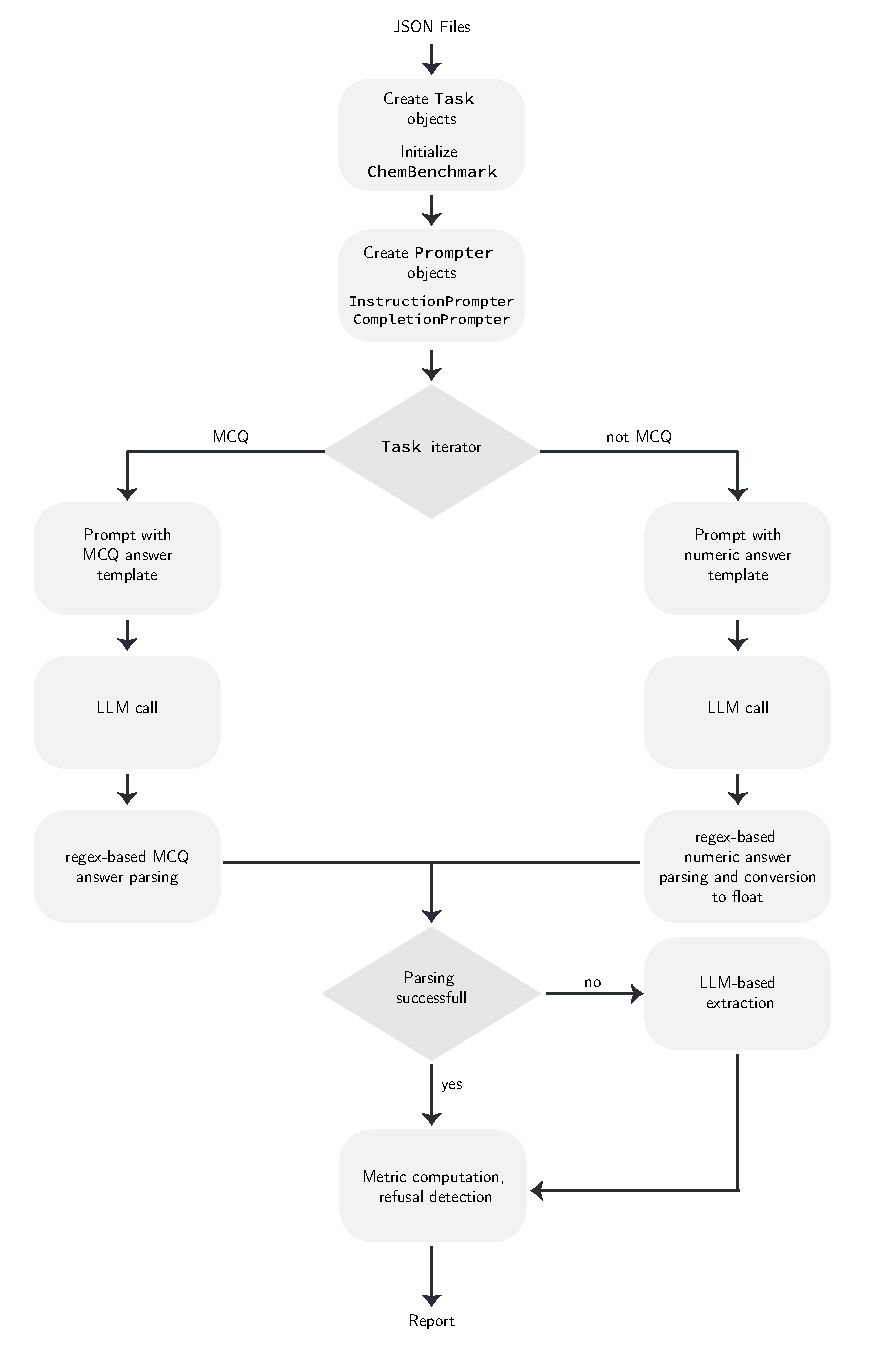
\includegraphics[height=.7\textheight]{figures/process.pdf}
    \caption{\textbf{Overview of the benchmarking pipeline implemented in \chembench.} The process begins with JSON files containing task data, which are used to create \texttt{Task} objects and initialize the \texttt{ChemBenchmark}. \texttt{Prompter} objects are then created to handle different types of prompts for instruction-tuned and completion models.
    The \texttt{Task} Iterator differentiates between \gls{mcq} and other question types. For each task type, appropriate prompts are generated and passed to the \gls{llm}. The responses are then processed using regex-based parsing methods specific to \gls{mcq} or numeric answers (after obtaining the relevant part of the response from the instruction-tuned models).
    The regex-based parsing is elaborate and also able to handle special cases such as scientific notation, or roman numerals.
    If the initial parsing is unsuccessful, the system employs an \gls{llm}-based extraction method as a fallback. The parsed or extracted answers then undergo metric computation and refusal detection.}
    \label{fig:process}
\end{figure}



\clearpage
\subsection{Human baseline} \label{sec:human_baseline}
\paragraph{App} To facilitate the collection of responses, we developed a responsive web application in Typescript using the Next.js\autocite{nextjs} app router framework.
This application handles serving the user interface and exposes various \gls{rest} \glspl{api} for relevant operations.
We utilize a Postgresql.
The web application is styled with Tailwind CSS\autocite{tailwindcss} using the shadcn/ui component library and uses NextAuth\autocite{nextauth} for easy and secure user authentication.
The application is hosted on the Vercel web hosting platform.

In the applications, human participants were presented with molecules as rendered drawings and SMILES strings. \LaTeX\xspace equations and chemical equations were rendered using MathJax (\Cref{fig:screenshots}).


\begin{figure}
    \subfloat[A physcial chemistry question.]{
        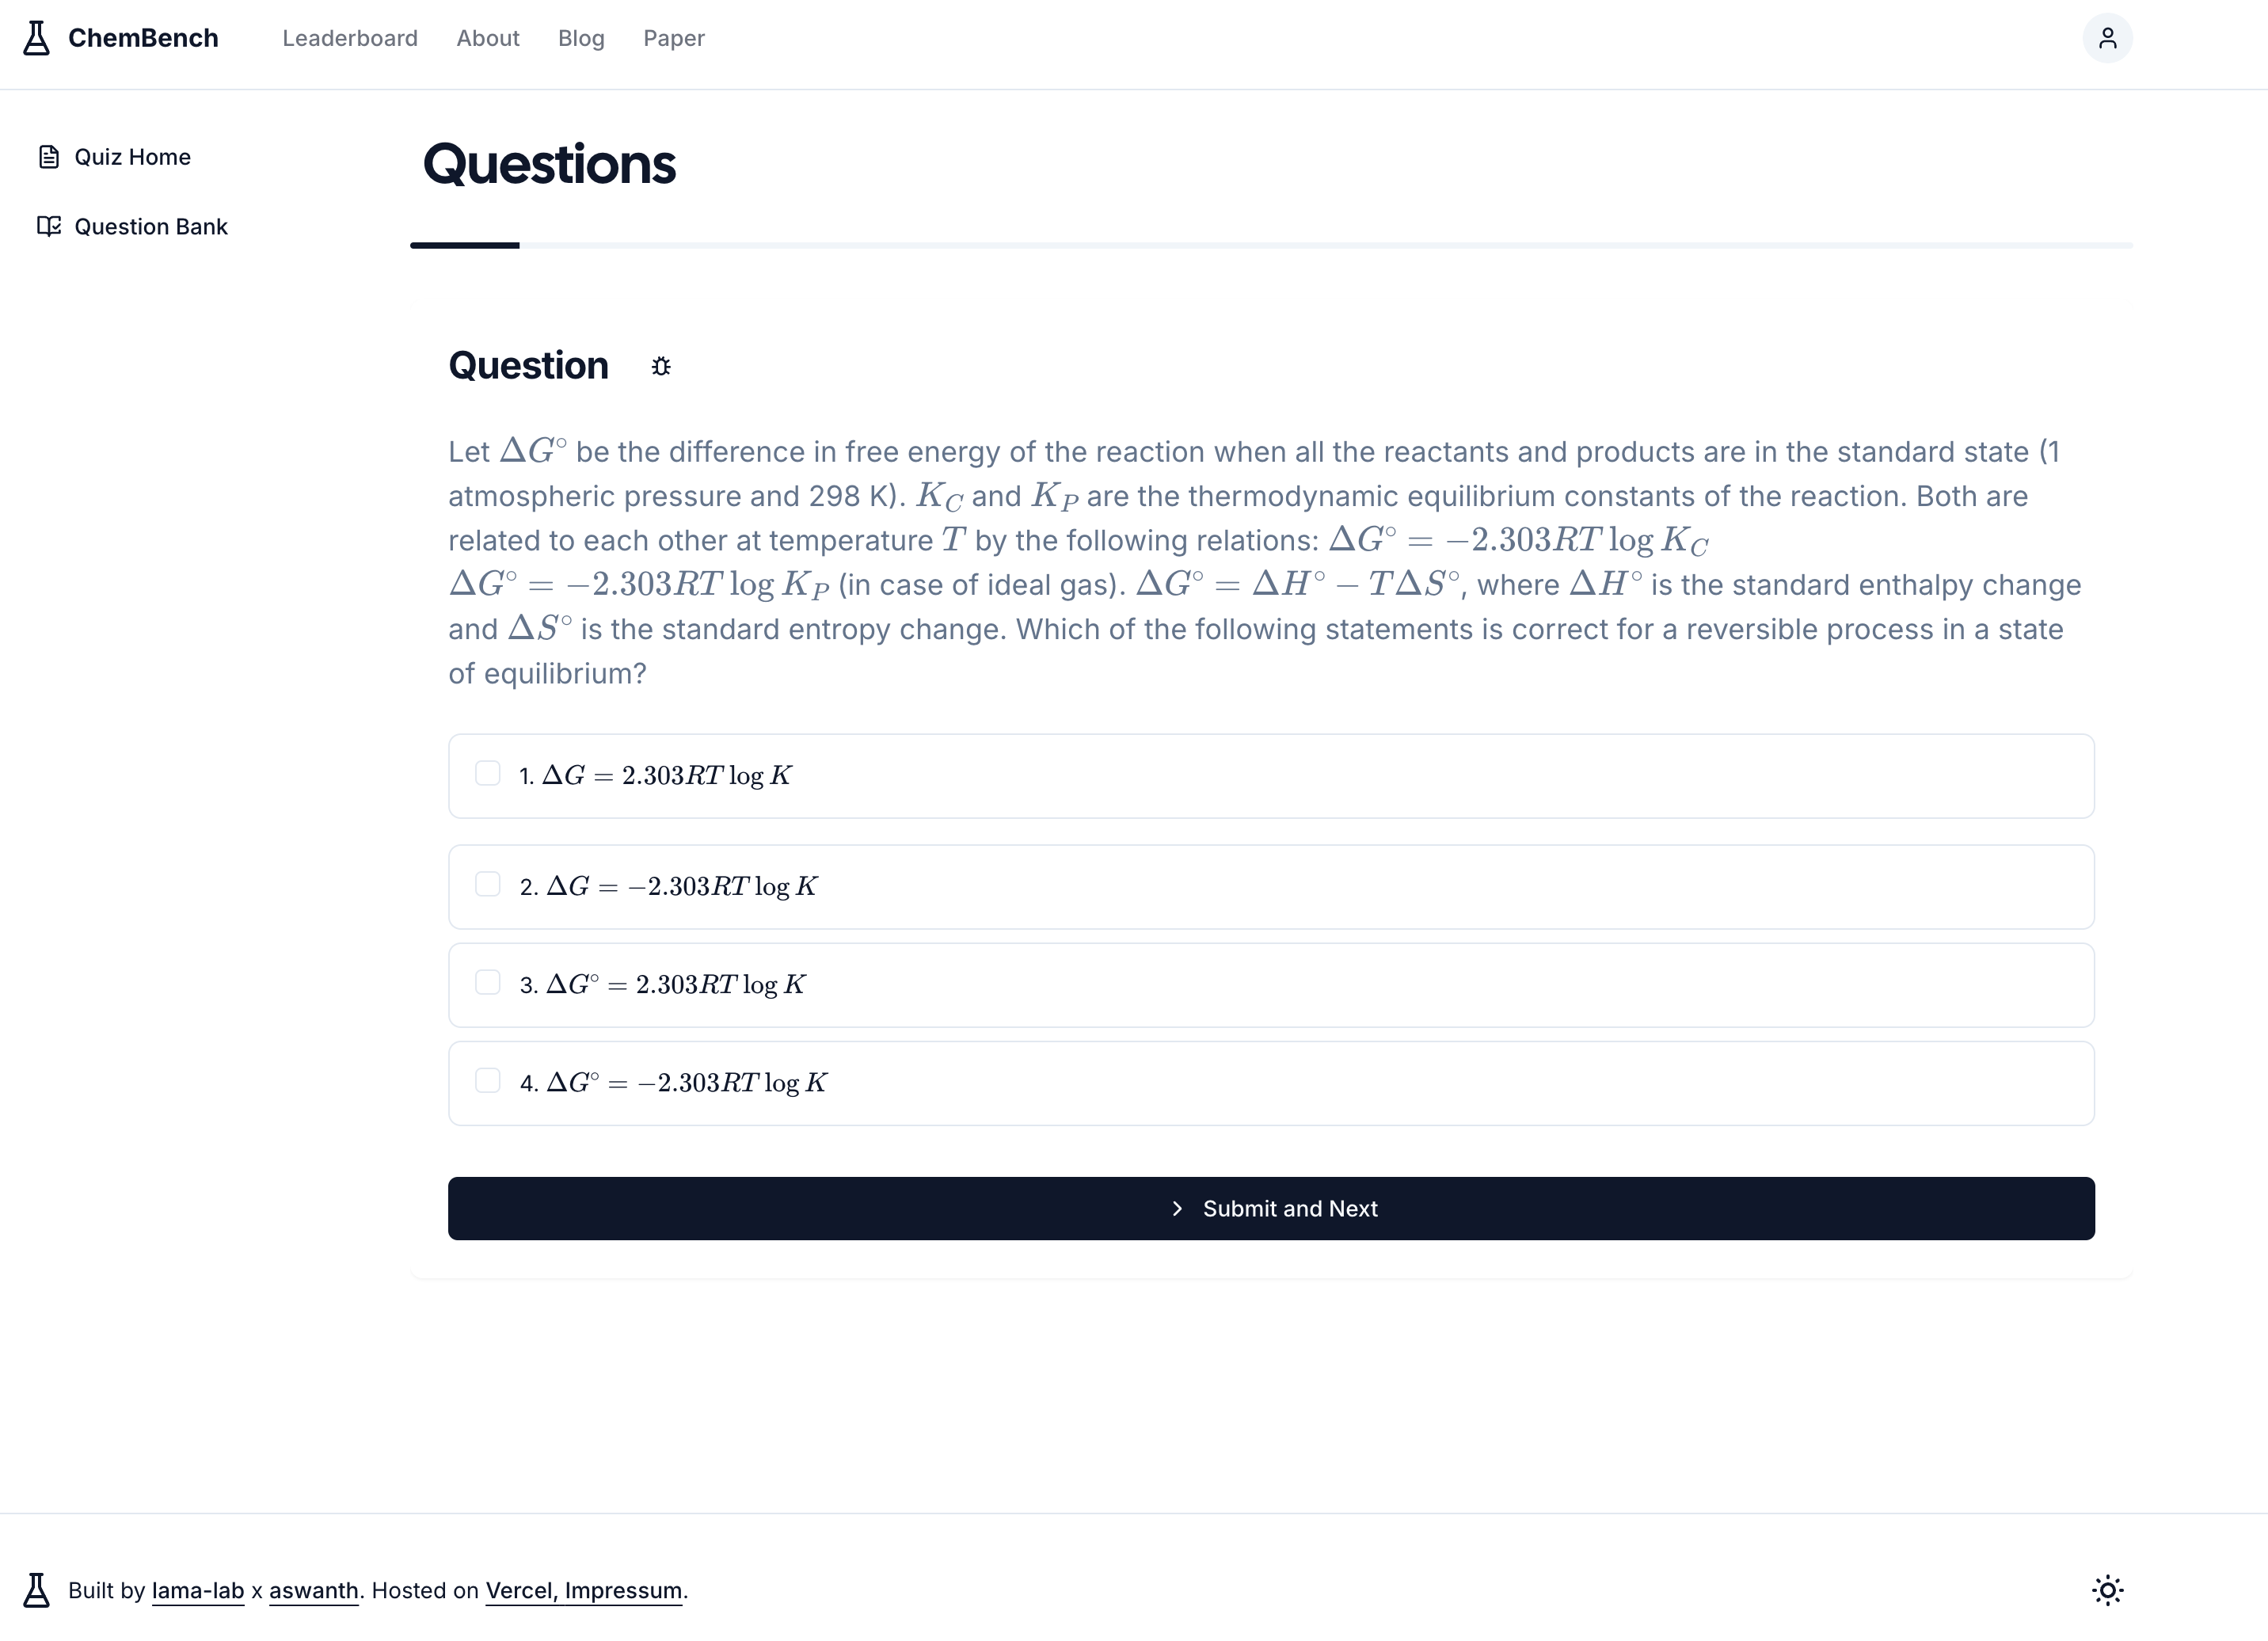
\includegraphics[width=\textwidth]{figures/screenshot_a.png}
    }

    \subfloat[An organic chemistry question.]{
        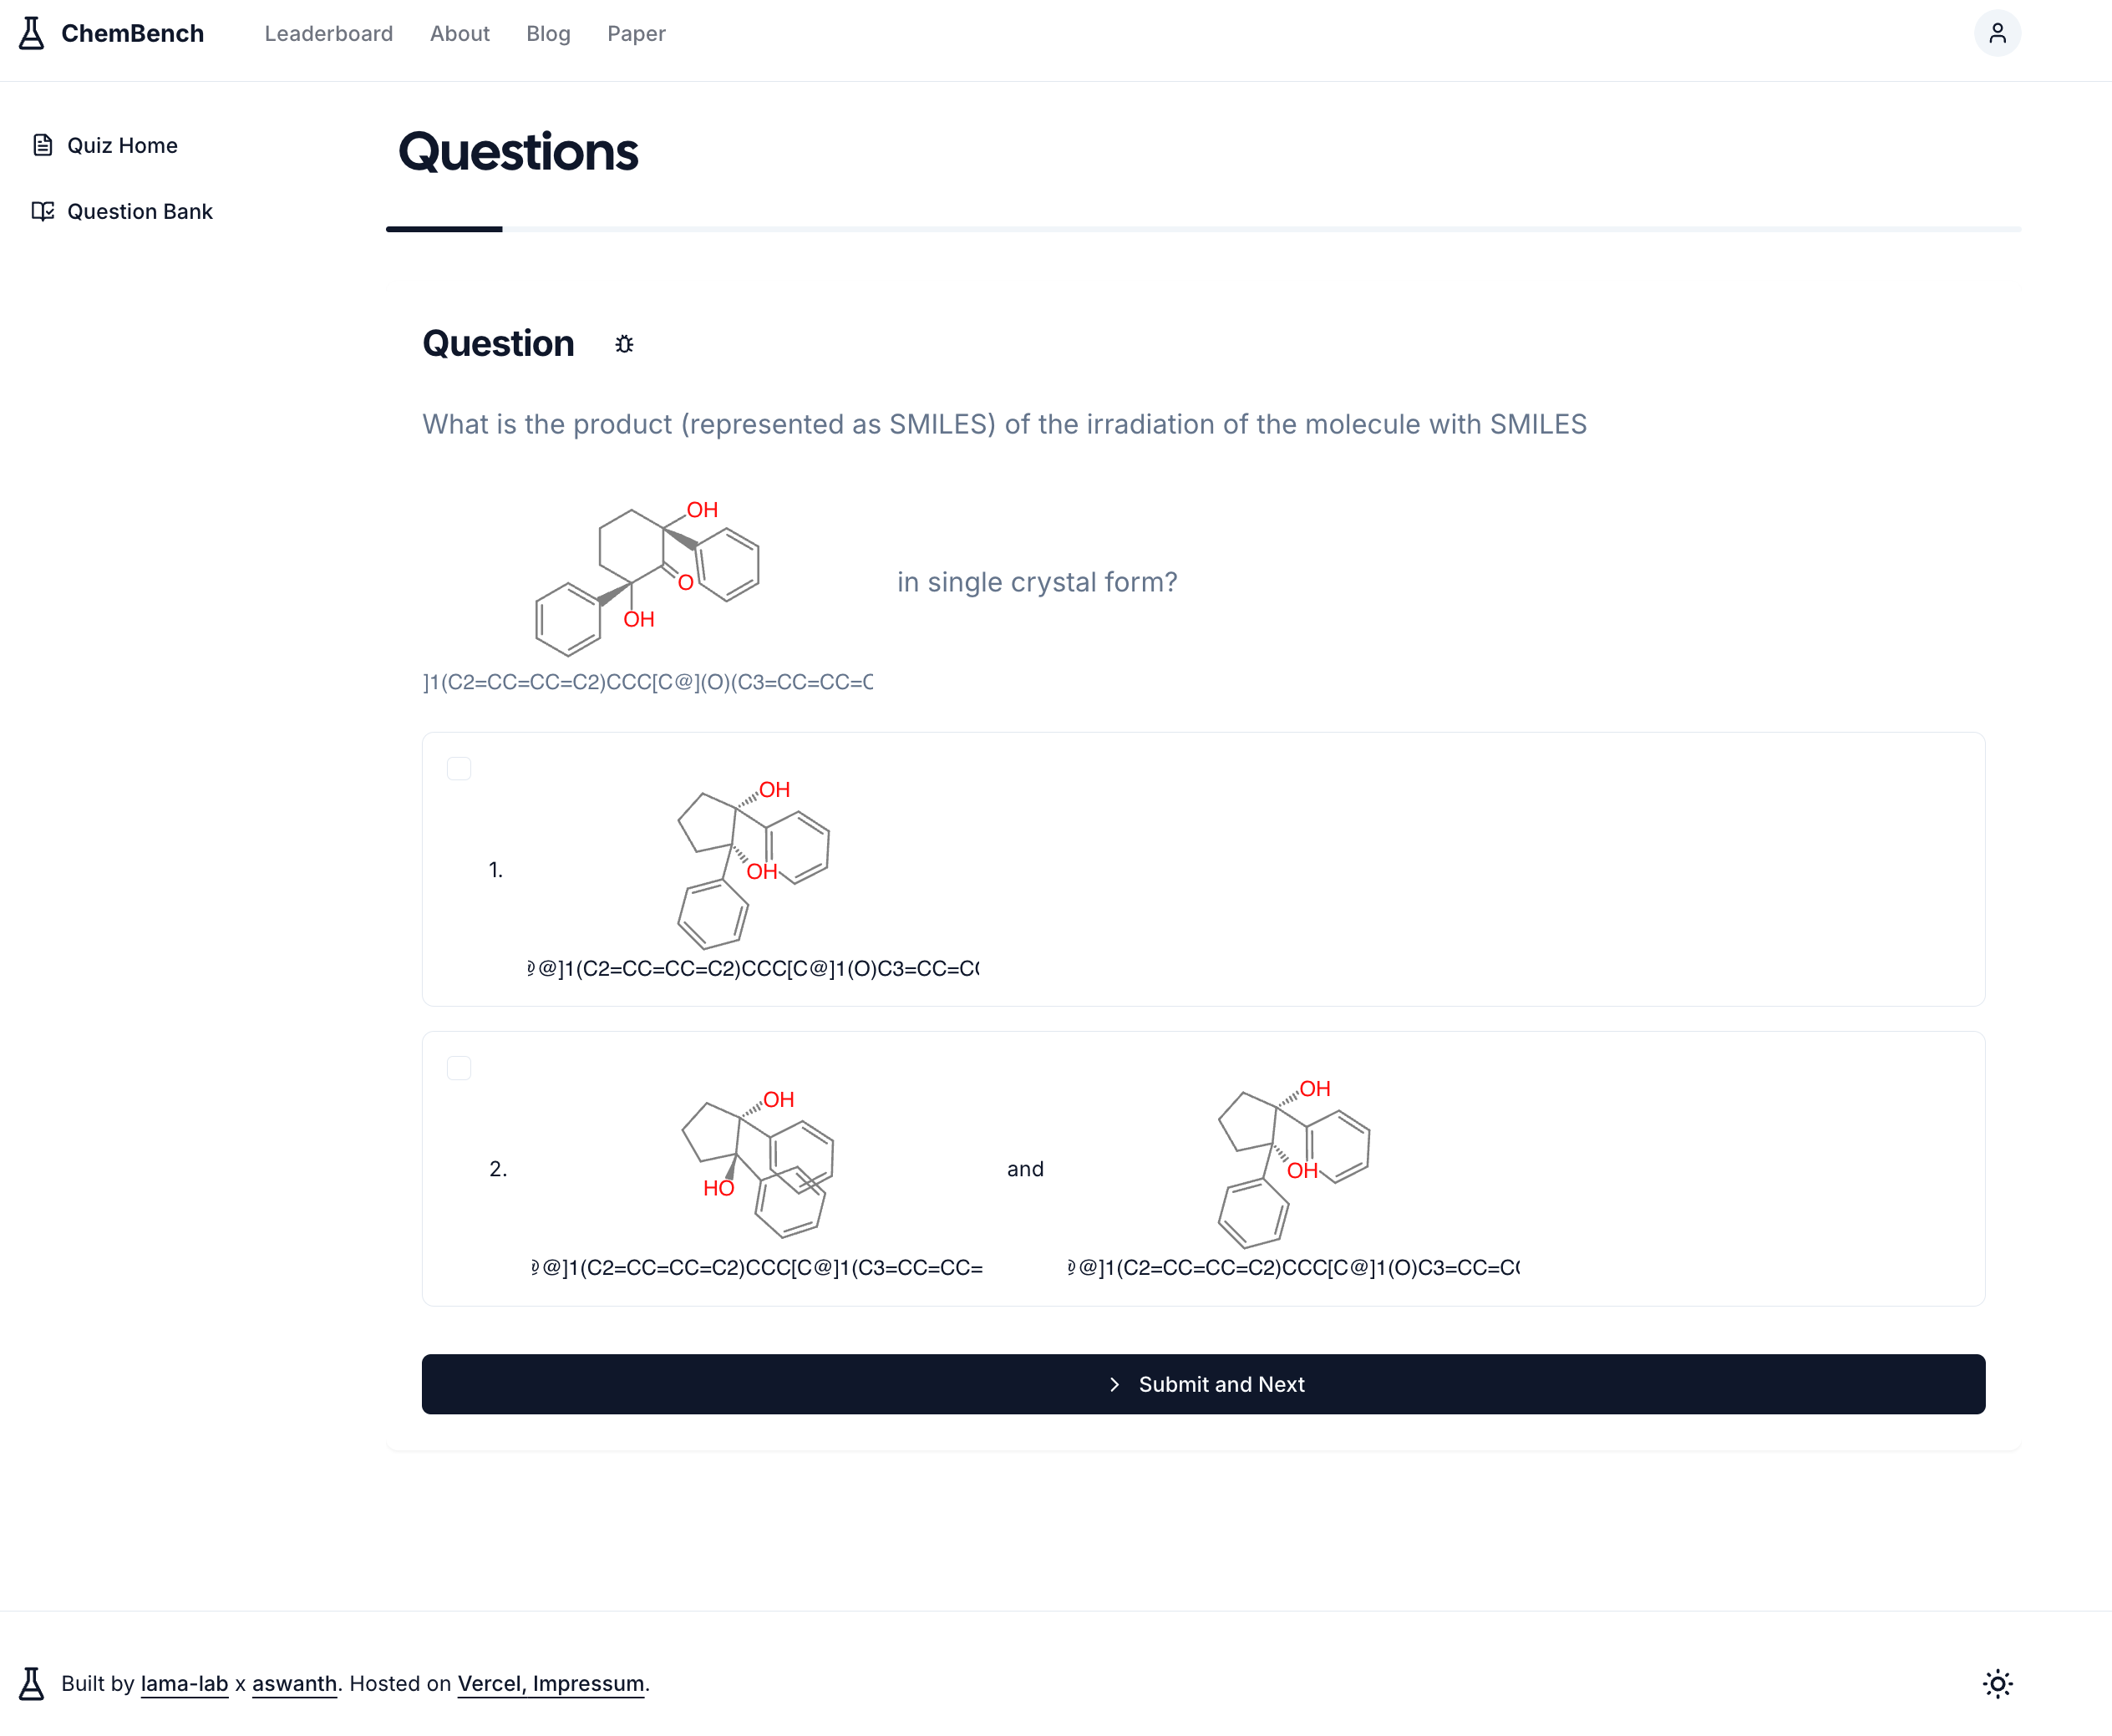
\includegraphics[width=\textwidth]{figures/screenshot_b.png}
    }
    \caption{\textbf{Examples of how questions were shown to the human participants.}}
    \label{fig:screenshots}
\end{figure}

\paragraph{Statistics}
\Cref{fig:human_score_distribution} shows the distribution of scores our human scorers achieved.

\begin{figure}[htb]
    \centering
    \includegraphics{figures/human_score_distribution.pdf}
    \script{plot_human_score_distribution.py}
    \caption{\textbf{Distribution of human scores.}The histogram and kernel density estimates show the fraction of questions answered correctly by the human volunteers.
    Since the best possible score for each question is one and the worst possible score is zero, the values on this plot are between zero and one. A score of one would mean that a volunteer answered all questions correctly. A score of zero would mean that no question was answered correctly. 
    We find that the scores for the questions that the human volunteers answered with tools are generally lower than the scores for the questions that the human volunteers answered without tools.}
    \label{fig:human_score_distribution}
\end{figure}

We also recorded the time humans took to answer the questions (\Cref{fig:human_timing}). This time is the time from the question being displayed to the human to the human submitting the answer.

\begin{figure}[htb]
    \centering
    \includegraphics{figures/human_timing.pdf}
    \script{analyze_human_data.py}
    \caption{\textbf{Time taken by human scorers to answer questions vs.\ correctness of their answers.} From the plot, it is clear that there is no clear dependence of the correctness of the answers on the time taken by the human scorers to answer the questions. However, we see that human scorers typically took longer to correctly answer questions with tool use.}
    \label{fig:human_timing}
\end{figure}

Additionally, we prompted users to provide additional information about their experience in chemistry.
While we recorded fine-grained information, e.g., their specialization, we focused on the number of years since the first university-level chemistry course.
\Cref{fig:experience_vs_correctness} shows that the experience of the human scorers was weakly correlated with the correctness of their answers (\Cref{fig:experience_vs_correctness}, Spearman's \(\rho \approx \variable{output/spearman_experience_score.txt}\), and \(p \approx \variable{output/spearman_experience_score_p.txt}\)).

\begin{figure}[htb]
    \centering
    \includegraphics{figures/experience_vs_correctness.pdf}
    \script{analyze_human_data.py}
    \caption{\textbf{Experience of human  scorers vs.\ correctness of their answers.} The experience (in the number of years since the first university-level chemistry course) of the human scorers wasp correlated with the correctness of their answers.}
    \label{fig:experience_vs_correctness}
\end{figure}

\paragraph{Tool use}
In our study, humans were allowed to use tools for answering some questions.
They could also report what tools they used for answering questions. As \Cref{fig:tool_use} shows, the most commonly tool was some form of web search (which, according to the freetext responses, often was a multi-step process).

\begin{figure}
    \centering
    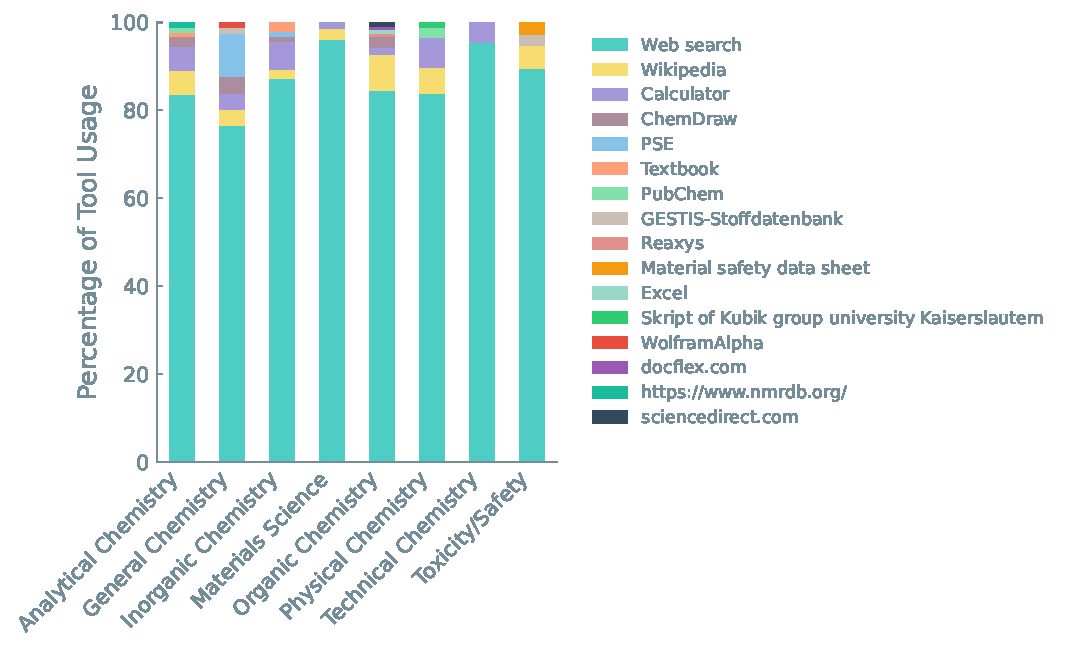
\includegraphics[width=\textwidth]{figures/human_tool_usage_by_topic.pdf}
    \script{human_tool_usage.py}
    \caption{\textbf{Tool usage by human scorers.} The plot shows the most commonly used tools by human participants.}
    \label{fig:tool_use}
\end{figure}

\clearpage
\subsection{Tool augmented models} \label{sec:react-environment}
In addition to directly prompting \glspl{llm}, we also investigated the performance of tool-augmented systems.
For this, we investigated the two models which showed the best overall results, \GPTFourO and \ClaudeThreeFiveSonnet (\oone overperformed both models but is not recommended using this model with such \enquote{reasoning} prompts such as ReAct\autocite{yao2022react} or \gls{cot}\autocite{wei2023cot}). 
For both models, we created a ReAct-style tool augmentation environment in which models had access to WolframAlpha, the ArXiv \gls{api}, Wikipedia, and web search (using Brave search \gls{api}).
We based the selection of these tools on the most used tools by humans (see \Cref{fig:tool_use}).
Additionally, we added two specific tools to convert \gls{iupac} names to \gls{smiles}, and \gls{smiles} to \gls{iupac} names.
These conversion tools allow us to better understand how the agents perform for some specific questions in this agent environment configuration.
We implemented the systems using Langchain\autocite{Chase_LangChain_2022} with the default ReAct prompt and constrained the system to a maximum of ten \gls{llm} calls.

While for \ClaudeThreeFiveSonnet the overall performance did not change, we observe a decrease in performance for \GPTFourO compared with the \llm without tools (\Cref{tab:performance_table}). 
If we study the results by each type of question, we observe an improvement for questions regarding electron counts or point groups of compounds.
However, the scores decreased for questions asking about the number of isomers or \gls{ghs} pictograms.
For the specific questions about converting \gls{iupac} names to \gls{smiles}, the results decreased notably despite the models having access to specific tools prepared for those questions. 
By studying the reasoning path for these cases, we found that the error results from the models responding in a format that the LangChain framework with the default ReAct loop cannot handle. 
This indicates that agent frameworks need optimization to be more robust. It involves not only equipping the \glspl{llm} with tools but also necessitates engineering efforts to create robust systems.


\clearpage
\subsection{Confidence estimates} \label{sec:confidence_estimates}

Since it is important to understand if models can provide an indication of whether their answer might likely be incorrect, we prompted some of our top performing \glspl{llm} to return the confidence in providing a correct answer on an ordinal scale.
This is similar to the verbalized confidence scores reported by \textcite{xiong2023llms}.
We find that the models show different distributions of confidence scores, which, for some, are skewed to the extremes.

In addition, we also analyzed the confidence estimated via the log probabilities of the answer tokens. This probability of a token given the context is not necessarily the same as the confidence in the correctness of the answer. However, it is still often used as a proxy.

Our analysis of both log probabilities and prompting confidence reveals distinct calibration behaviors across different language models.
\GPTFourO demonstrates an overconfident tendency, often assigning high probabilities even to incorrect answers.
However, when \GPTFourO displays high confidence, it accurately predicts correct answers approximately \SI{80}{\percent} of the time. In contrast, \LlamaThreeOneEightBInstruct confidence distribution is more evenly spread, with a majority of predictions centered around 0.5. High-confidence predictions from \LlamaThreeOneEightBInstruct are less frequent compared to \GPTFourO, and unlike \GPTFourO, high confidence does not necessarily correlate with a higher chance of correct answers.

\begin{figure}[htb]
    \centering
    \includegraphics[width=\textwidth]{figures/log_probs_calibration_plot_overall_filtered.pdf}
    \caption{\textbf{Reliability diagram of histogram of logit-based confidence estimates.} For this analysis we obtained the linear probability from the logprobs of the models. Only logprobs of the tokens corresponding to the answers were considered. Linear proabability was computed by taking exponential of logprobs (for sequences with multiple tokens, values were multiplied).  The plot shows the average predicted probability and the fraction of correct answers for each bin of linear probabilities. The ideal scenario is a diagonal line, indicating perfect calibration where the model's confidence aligns perfectly with the actual correctness. The \gls{ece} value quantifies the overall calibration performance, with a lower \gls{ece} indicating better calibration.}
    \label{fig:confidence_score_distributions}
    \script{plot_logprobs.py}
\end{figure}

\clearpage
\subsection{Impact of sampling temperature}
We also investigated the impact of sampling temperature (i.e. temperature 0 means always sampling the most likely token, higher temperatures introduce some randomness in the generation process) on the performance of the models. \Cref{fig:temperature_impact} shows that, generally, the performance of models tends to decrease with increasing temperature.

\begin{figure}[!h]
    \centering
    \includegraphics{figures/swarm_plot_combined.pdf}
    \caption{\textbf{Impact of sampling temperature on the performance of the models.} The plot shows the performance of the models at zero temperature (i.e., greedy decoding) and temperature of one. The performance is measured in terms of the fraction of questions answered correctly.}
    \label{fig:temperature_impact}
    \script{plot_temperature_diffs.py}
\end{figure}


\clearpage
\subsection{Summary of trends and recommendations}

\oone consistently leads across both the \ChemBench corpus and \chembenchmini.  \ClaudeThreeFiveSonnet, \GPTFourO, \LlamaThreeOneFourZeroFiveBInstruct form the next tier of strong performers. These models show robust performance across all skills and difficulty levels. 

Larger models generally perform better (\LlamaThreeOneFourZeroFiveBInstruct > \LlamaThreeOneSeventyBInstruct > \LlamaThreeOneEightBInstruct). However, smaller but well-designed models can compete with larger models. For example, \GemmaTwoNineBIt has an overall accuracy of \variable{output/trends_section_variables/gemma_9B.txt} on the \ChemBench corpus, which is only \variable{output/trends_section_variables/diff_between_llama_405B_and_gemma_9B.txt}\% less accurate than the much larger \LlamaThreeOneFourZeroFiveBInstruct model.

One can observe a clear progression of performance across model families (e.g., \ClaudeThreeFiveSonnet >  \ClaudeThree > \ClaudeTwo or \GPTFourO > \GPTFour > \GPTThreeFiveTurboZeroT). Newer versions consistently outperform their predecessors.
Scores on knowledge-intensive tasks are typically lower than those on calculation and reasoning-intensive questions. 

Based on these findings, some scope for improving these models could be to focus on enhancing knowledge-based training, possibly through improved pre-training on chemistry-specific texts or with chemistry knowledge-base integration. However, innovation is also needed to incorporate this information into the systems. For example, even \PaperQATwo could not outperform the \gls{llm} it is using for directing the tools, even though the agent has access to literature evidence.
This suggests we might need to not only focus on building chemistry-specific retrieval datasets since current systems fail to retrieve the relevant papers and should be coupled with more domain-specific databases. However, the observation that our ReAct agents were too fragile to answer questions for which they had custom-made tools available correctly suggests that we also must invest in building more robust agent frameworks (see \Cref{sec:react-environment} for further discussion about the ReAct environment). 

Models show the strongest performance in reasoning tasks on the \chembench corpus, which suggests that current training approaches are good at developing logical/reasoning capabilities for basic problem-solving of university-level exams. However, performance drops significantly for advanced tasks, suggesting that more advanced chemistry problems with complex, multi-step solutions (e.g., solving analytical chemistry problems) should be included in training or finetuning.

The post-training (e.g., \gls{rlhf}) of the current models does not equip them with human-like \enquote{chemical taste.} This, however, will be essential for future discovery research (e.g., in combination with genetic algorithms).

\clearpage
\subsection{Leaderboard}
\label{sec:leaderboard}
Our leaderboard is based on the tool chain developed for Matbench.\autocite{Dunn_2020}
Briefly, the \chembench pipeline produces standardized files in \texttt{json} format that contributors can add via pull requests to the \chembench repository.
The Markdown tables and interactive plots are automatically generated and updated on the \chembench website. The leaderboard is available at \url{https://lamalab-org.github.io/chem-bench/leaderboard/}.

\clearpage

\printnoidxglossary[type=\acronymtype, nonumberlist]  % https://github.com/tectonic-typesetting/tectonic/issues/704
